\subsection{NEON}
\subsubsection{Function Analysis}
To implement NEON version of \textit{gaussian\_smooth} function, the feature of the function is analyzed first to determine how NEON can be utilized to
realize the function. In this function, blurring operations are performed twice, the first operation is based on x direction and the other is based on y direction of the image. Due to the similarity of the operations, only the first operation is analyzed in this section. 

The nature of Gaussian blur is to convolve the image with Gaussian function. In the original program, the Gaussian filter, which is called kernel in the application, has 15 Gaussian values to blur a single pixel. This implementation illustrates that 7 neighbor values on both sides of a pixel, and the value of the pixel itself are taken to do the calculation. In C code, the calculation is executed by using for-loop iteration for each value. While in the NEON implementation, we decided to take the advantage of parallel computing of NEON; calculating multiple values at the same time.

\subsubsection{Gaussian Algorithm}
In \textit{gaussian\_smooth} function, the blurred value are stored in single-precision floating-point. For NEON, four same operations based on single-precision floating-point can be performed simultaneously. Since the number of Gaussian values is not a multiple of 4, we decided to have some modifications to implement the operation on NEON. 

Originally, 7 neighbor values are taken on either side of a pixel. In our case, we decided to take values from 8 neighbors (two times of NEON calculation)for calculating simplicity. However, in order to coincide with the original calculation, the corresponding Gaussian value of newly added neighbors are set to 0 to ensure they do not affect the calculation output at the end. In the implementation, we take an extra value at both the left-most side and right-most side of the neighbor, and adding two extra zeros at both the head and tail of the Gaussian filter. Figure~\ref{fig:newfilter} shows how the Gaussian kernel is modified and split for NEON implementation. Different from other Gaussian values, kernel[8] is used separately for the calculation of the pixel itself. 

\begin{figure}
\centering
%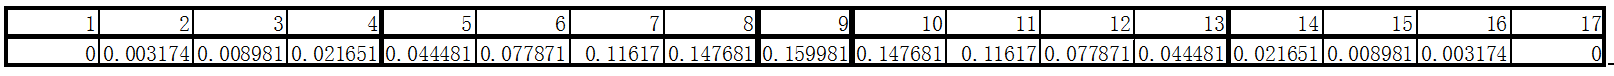
\includegraphics[width=0.4\textwidth]{drawings/filter}
\caption{Modified Filter}
\label{fig:newfilter}
\end{figure}
